
%% bare_conf.tex
%% V1.3
%% 2007/01/11
%% by Michael Shell
%% See:
%% http://www.michaelshell.org/
%% for current contact information.
%%
%% This is a skeleton file demonstrating the use of IEEEtran.cls
%% (requires IEEEtran.cls version 1.7 or later) with an IEEE conference paper.
%%
%% Support sites:
%% http://www.michaelshell.org/tex/ieeetran/
%% http://www.ctan.org/tex-archive/macros/latex/contrib/IEEEtran/
%% and
%% http://www.ieee.org/

%%*************************************************************************
%% Legal Notice:
%% This code is offered as-is without any warranty either expressed or
%% implied; without even the implied warranty of MERCHANTABILITY or
%% FITNESS FOR A PARTICULAR PURPOSE! 
%% User assumes all risk.
%% In no event shall IEEE or any contributor to this code be liable for
%% any damages or losses, including, but not limited to, incidental,
%% consequential, or any other damages, resulting from the use or misuse
%% of any information contained here.
%%
%% All comments are the opinions of their respective authors and are not
%% necessarily endorsed by the IEEE.
%%
%% This work is distributed under the LaTeX Project Public License (LPPL)
%% ( http://www.latex-project.org/ ) version 1.3, and may be freely used,
%% distributed and modified. A copy of the LPPL, version 1.3, is included
%% in the base LaTeX documentation of all distributions of LaTeX released
%% 2003/12/01 or later.
%% Retain all contribution notices and credits.
%% ** Modified files should be clearly indicated as such, including  **
%% ** renaming them and changing author support contact information. **
%%
%% File list of work: IEEEtran.cls, IEEEtran_HOWTO.pdf, bare_adv.tex,
%%                    bare_conf.tex, bare_jrnl.tex, bare_jrnl_compsoc.tex
%%*************************************************************************

% *** Authors should verify (and, if needed, correct) their LaTeX system  ***
% *** with the testflow diagnostic prior to trusting their LaTeX platform ***
% *** with production work. IEEE's font choices can trigger bugs that do  ***
% *** not appear when using other class files.                            ***
% The testflow support page is at:
% http://www.michaelshell.org/tex/testflow/



% Note that the a4paper option is mainly intended so that authors in
% countries using A4 can easily print to A4 and see how their papers will
% look in print - the typesetting of the document will not typically be
% affected with changes in paper size (but the bottom and side margins will).
% Use the testflow package mentioned above to verify correct handling of
% both paper sizes by the user's LaTeX system.
%
% Also note that the "draftcls" or "draftclsnofoot", not "draft", option
% should be used if it is desired that the figures are to be displayed in
% draft mode.
%
\documentclass[10pt, conference, compsocconf]{IEEEtran}
% Add the compsocconf option for Computer Society conferences.
%
% If IEEEtran.cls has not been installed into the LaTeX system files,
% manually specify the path to it like:
% \documentclass[conference]{../sty/IEEEtran}

% *** GRAPHICS RELATED PACKAGES ***
%
\usepackage[pdftex]{graphicx}
\graphicspath{{images/}}
\DeclareGraphicsExtensions{.pdf,.jpeg,.png}

% *** MATH PACKAGES ***
\usepackage{amssymb}
\usepackage{amsmath}
\usepackage{xcolor}
\usepackage{url}
\usepackage{algorithmicx}
\usepackage{algpseudocode}

\newcommand{\todo}[1]{\texttt{\textcolor{red}{#1}}}

% *** ALIGNMENT PACKAGES ***
%
%\usepackage{array}
% Frank Mittelbach's and David Carlisle's array.sty patches and improves
% the standard LaTeX2e array and tabular environments to provide better
% appearance and additional user controls. As the default LaTeX2e table
% generation code is lacking to the point of almost being broken with
% respect to the quality of the end results, all users are strongly
% advised to use an enhanced (at the very least that provided by array.sty)
% set of table tools. array.sty is already installed on most systems. The
% latest version and documentation can be obtained at:
% http://www.ctan.org/tex-archive/macros/latex/required/tools/


%\usepackage{mdwmath}
%\usepackage{mdwtab}
% Also highly recommended is Mark Wooding's extremely powerful MDW tools,
% especially mdwmath.sty and mdwtab.sty which are used to format equations
% and tables, respectively. The MDWtools set is already installed on most
% LaTeX systems. The lastest version and documentation is available at:
% http://www.ctan.org/tex-archive/macros/latex/contrib/mdwtools/


% IEEEtran contains the IEEEeqnarray family of commands that can be used to
% generate multiline equations as well as matrices, tables, etc., of high
% quality.


%\usepackage{eqparbox}
% Also of notable interest is Scott Pakin's eqparbox package for creating
% (automatically sized) equal width boxes - aka "natural width parboxes".
% Available at:
% http://www.ctan.org/tex-archive/macros/latex/contrib/eqparbox/


% *** Do not adjust lengths that control margins, column widths, etc. ***
% *** Do not use packages that alter fonts (such as pslatex).         ***
% There should be no need to do such things with IEEEtran.cls V1.6 and later.
% (Unless specifically asked to do so by the journal or conference you plan
% to submit to, of course. )


% correct bad hyphenation here
\hyphenation{op-tical net-works semi-conduc-tor}

\DeclareMathOperator*{\argmin}{arg\!\min}
\begin{document}
%
% paper title
% can use linebreaks \\ within to get better formatting as desired
\title{Practical Distributed Classification using the\\ Alternating Direction Method of Multipliers Algorithm}


% author names and affiliations
% use a multiple column layout for up to two different
% affiliations

\author{\IEEEauthorblockN{Peter Lubell-Doughtie and Jon Sondag}
\IEEEauthorblockA{Intent Media\\
New York, USA\\
\{peter.lubell-doughtie, jon.sondag\}@intentmedia.com}
}

% conference papers do not typically use \thanks and this command
% is locked out in conference mode. If really needed, such as for
% the acknowledgment of grants, issue a \IEEEoverridecommandlockouts
% after \documentclass

% use for special paper notices
%\IEEEspecialpapernotice{(Invited Paper)}




% make the title area
\maketitle


\begin{abstract}
We describe a specific implementation of the Alternating Direction Method of Multipliers (ADMM) algorithm for distributed optimization.  The implementation runs logistic regression with L2 regularization over large datasets and does not require a user-tuned learning rate metaparameter.  Throughout we emphasize the practical lessons learned while implementing an iterative MapReduce algorithm and the advantages of remaining within the Hadoop ecosystem.
\end{abstract}

\begin{IEEEkeywords}
distributed algorithms; distributed computing; optimization; predictive models
\end{IEEEkeywords}


% For peer review papers, you can put extra information on the cover
% page as needed:
% \ifCLASSOPTIONpeerreview
% \begin{center} \bfseries EDICS Category: 3-BBND \end{center}
% \fi
%
% For peerreview papers, this IEEEtran command inserts a page break and
% creates the second title. It will be ignored for other modes.
\IEEEpeerreviewmaketitle



\section{Introduction}
When used at scale, statistical modeling algorithms need to function correctly on large amounts of data in a practical amount of time.  In many cases production-scale datasets do not fit into the memory available on a single machine and the dataset needs to be distributed over a cluster.

The MapReduce programming model \cite{dean2004} allows clients to run computations on large distributed datasets with commodity machines.  Apache Hadoop is a well known, widely used, and broadly supported MapReduce platform which works with the Hadoop Distributed File System (HDFS)  and supports arbitrarily large datasets \cite{white2009}.

The ADMM algorithm \cite{boyd} is a distributed convex optimization algorithm that can be used to fit machine learning models with convex loss---including linear regression, logistic regression, and support vector machines---and L1 or L2 parameter regularization.  We choose to implement ADMM using Hadoop in order to benefit from the wealth of existing Hadoop utilities and the community's extensive knowledge.

Regardless of the problems concerning Hadoop's support for iteration \cite{bu2010}, we show that Hadoop can be used to implement an efficient iterative algorithm which is ``good enough'' in the sense of \cite{lin2012}.  That is to say, the benefits of using a reliable platform that easily integrates with our existing toolset outweigh the small increase in time per job.  To support iteration within Hadoop, we write data from external storage to HDFS to reduce network latency when transferring large amounts of data.  We also use Hadoop's \emph{Input Splits} to persistently partition data between mappers over multiple iterations. 

Many challenging problem domains, for example click attribution in online advertising, involve noisy observations of sparse data.  Modeling in these domains requires significant amounts of data and an interpretable model.  Here we focus on logistic regression with L2 norm.

Traditional batch optimization algorithms for logistic regression fit the model parameters iteratively and require that the training dataset fit into memory for good performance. ADMM also proceeds iteratively but solves an intermediate optimization problem in parallel on subsets of the training data, then combines the intermediate solutions to find a consensus result at each iteration. The time-consuming and memory-intensive intermediate optimization problems are solved in parallel.

When executing long-running modeling jobs hand-tuning parameters can be especially time-consuming.  To avoid this, we use ADMM with methods that automatically tune parameters while still guaranteeing convergence.  This makes for an easy transition from small-scale prototypes fit using batch optimization methods on a sample of the dataset, to large-scale models fit over the entire dataset.

Our main contribution is an adaptation of ADMM that makes large-scale logistic regression user-friendly on a single popular platform.  Using our implementation, data scientists can accurately fit models without tuning meta-parameters.

The rest of the paper is organized as follows.  In section \ref{sec:prob} we formulate logistic regression using the ADMM algorithm, then in section \ref{sec:imp} we provide details concerning how to implement the ADMM algorithm in Hadoop MapReduce.  In section \ref{sec:results} we present the results of running ADMM on a production scale dataset.  In section \ref{sec:related} we review recent work related to iterative optimization with Hadoop, and in section \ref{sec:conc} we conclude.

\section{Problem Formulation}\label{sec:prob}

In this section we describe exactly how we formulate regularized Logistic Regression with ADMM. Given a matrix of features $\mathbf{A}\in\mathbf{R}^{m\times n}$ and a vector of their labels $b\in\mathbf{R}^m$ with $b_i\in\{-1,1\}$, our goal is to compute the probability $\text{Pr}(b_i=1|\mathbf{A}_i)$ for each row $1\leq i\leq m$.  The first column of the feature matrix represents the intercept and all values in this column are set to 1.

In general, the (not necessarily distributed) convex model fitting problem with regularization can be written as:
\begin{align*}
\text{minimize}&\quad \dfrac{1}{m}\sum_{i=1}^m l_i(\mathbf{A}_i^Tx - b_i) + r(x),
\end{align*}
where $l_i$ is the loss for training example $i$, $r$ is a regularization term, and $x\in\mathbf{R}^n$ is the vector that solves the optimization problem and defines the logistic regression model.

In the case of L2 regularized logistic regression the problem becomes:
\begin{align*}
\text{minimize}&\quad \dfrac{1}{m}\sum_{i=1}^m \log(1 + exp(-b_i\mathbf{A}_i^Tx)) + \lambda\|x\|_2^2,
\end{align*}
where $\lambda$ is the regularization factor.

Rephrasing in ADMM global consensus form and reflecting the partitioning of training examples across $N$ machines in the cluster, the problem becomes:
\begin{align*}
\text{minimize}&\quad \dfrac{1}{m}\sum_{i_1=1}^{m_1} \log(1 + exp(-b_{i_1}\mathbf{A}_{i_1}^Tx_{_1}))+\ldots \\
&\quad+\dfrac{1}{m}\sum_{i_N=1}^{m_N} \log(1 + exp(-b_{i_N}\mathbf{A}_{i_N}^Tx_{_N}))+\lambda\|z\|_2^2\\
\text{subject to}&\quad x_{_j} - z = 0, j = 1, \ldots, N
\end{align*}
where $x_{_j}\in\mathbf{R}^n$ is the logistic regression fit on machine $j$ and $z\in\mathbf{R}^n$ is a variable representing the global consensus.  After running the algorithm, $z$ is the vector of parameters that defines the model. The constraint, $x_j-z=0$, enforces equality of the parameter estimates across machines.

The ADMM algorithm for the above problem is:
\begin{align}
\label{eq:x}
x_{_j}^{k+1} :=&\quad \argmin_{x_{_j}} \dfrac{1}{m_j}\sum_{i_j=1}^{m_j} \log(1 + exp(-b_{i_j}\mathbf{A}_{i_j}^Tx_{_j})) \\
&\quad\quad\quad+ \dfrac{\rho^k}{2}\|x_{_j} - z^k + u_{_j}^k\|_2^2 \nonumber\\
\nonumber\\
\label{eq:z}
z^{k+1} :=&\quad \begin{cases}
    \bar{x}_q^{k+1} + \bar{u}_q^k& \text{if $q=1$}\\
    \\
    \dfrac{N\rho}{2\lambda + N\rho}(\bar{x}_q^{k+1} + \bar{u}_q^k)& \text{otherwise}
  \end{cases}\\
\nonumber\\
\label{eq:u}
u_j^{k+1} :=&\quad u_j^k + x_j^{k+1} - z^{k+1},
\end{align}
where $k$ is the iteration number, $\rho^k$ is the penalty parameter (see Section III) for iteration $k$, and $\bar{x}_q$ represents the average across all mappers of the $q$th element of the vector $\bar{x}\in\mathbf{R}^n$.  Formally, $\bar{x}_q = \dfrac{1}{N}\sum_{j=1}^N x_{q_j}$, and similarly for $\bar{u}$.  The first elements of $\bar{x}$ and $\bar{u}$, $\bar{x}_1$ and $\bar{u}_1$, correspond to the intercept and are not regularized, therefore we must treat them differently from the other values in the vector.

For each mapper $j$, $\mathbf{A}_{i_j}$ and $b_{i_j}$ are the portion of the data assigned to and used in that mapper.  The values of the $x_{_j}$ are calculated in parallel on the mappers while the values of $z$ and $u$ are calculated on the reducer.  The convex minimization problem for each $x_{_j}$ update is solved using the L-BFGS (low-memory BFGS) method \cite{bonnans2003numerical}.  We use a Java implementation of L-BFGS which is self contained and has performed well on Hadoop nodes.\footnote{\url{https://code.google.com/p/vladium/}}

\section{Implementation}\label{sec:imp}
In this section we describe implementing ADMM for Hadoop MapReduce and provide practical details relevant to using it to build models in a production environment.  The MapReduce model divides into three phases: the map, the shuffle, and the reduce.  In the map phase the input data is split among a set of mappers and each mapper applies a function to the set of data assigned to it.  In the shuffle phase the output of the mappers is assigned to a reducer.  In the reduce phase the mapper output is aggregated to create the final values, which are then output by the reducer.

The map and reduce steps can be expressed as:
\begin{alignat*}{2}
&\text{map}\quad &(k_1,v_2)\quad\rightarrow &\texttt{list}(k_2,v_2)\\
&\text{reduce}\quad &(k_2,\texttt{list}(v_2))\quad\rightarrow &\texttt{list}(v_2),
\end{alignat*}
where each mapper has a unique key, $k_1$.  The shuffle is concerned with mapping the intermediate key-value pairs, $(k_2,v_2)$, output by the mappers to the reducers \cite{dean2004}.

To implement MapReduce in Hadoop we define classes for the mapper and the reducer, along with a driver that handles input arguments and specifies the mapper and reducer classes (the shuffle is handled internally by Hadoop).  In the context of ADMM, each mapper performs the resource intensive task of computing the current $x_{_j}$.  After all mappers have completed their computations, we use a single reducer to compute the $z$ and $u_{_j}$ updates.

\subsection{Peristent Data with Input Splits}
When each mapper calculates the $x_{_j}^{k+1}$ values on iteration $k+1$, it must use the $u_{_j}^k$ values that were calculated for the same mapper in the previous iteration, $k$.  Hadoop does not normally accommodate this sort of persistence.  \cite{boyd} suggests using Apache HBase, a distributed data store, however this would add a new component and its accompanying complexity to the modeling framework.

As an alternative, we use Hadoop's notion of input splits to associate the correct $x_{_j}$ and $u_{_j}$ values with eachother, and with the location on HDFS of the data that they correspond to.  Input splits specify a \emph{split length} and a \emph{split ID}, which determine the size of the split data and the node on which to perform computations on that data, respectively.  To ensure that the correct $u_{_j}$ values are loaded when calculating an $x_{_j}$ value, the mapper reads the split ID and chooses the $u_i$ values based on this split ID.  The $z$ values are the same in each $x_{_j}$ formula, i.e. across mappers, and we simply replicate the current $z$ values across all mappers at the start of each iteration.

\subsection{Automatically Updating $\rho$}

We use the reducer to update the penalty parameter $\rho$.  The number of iterations before convergence depends upon the $\rho$ parameter, and hand-tuning $\rho$ can take a significant amount of time.  This is because we must wait for the algorithm to complete before determining the efficacy of the chosen $\rho$.

By varying the penalty parameter we can reduce the performance impact of our initial choice of $\rho$, and avoid spending time hand-tuning $\rho$.  We use the update scheme suggested in \cite{boyd} to update $\rho$ on each iteration:
\begin{equation}
\rho^{k+1}:=\begin{cases}
  \tau^{\text{incr}}\rho^k&\quad \text{if $\|r^k\|_2>\mu\|s^k\|_2$}\\
  \rho^k/\tau^{\text{decr}}&\quad \text{if $\|s^k\|_2>\mu\|r^k\|_2$}\\
  \rho^k&\quad \text{otherwise,}
\end{cases}
\label{eq:r}
\end{equation}
where $r^k$ is the primal residual, $s^k$ is the dual residual, and $\mu>1$, $\tau^{\text{incr}}>1$, and $\tau^{\text{decr}}>1$ are user-specified parameters.  We have used the typical values of $\mu=10$ and $\tau^{\text{incr}}=\tau^{\text{decr}}=2$.

\subsection{Considerations for MapReduce}
\begin{figure}
\begin{algorithmic}[1]
\Procedure {ADMM}{$\mathbf{A}$, $b$, $N$, $maxIterations$}
  \State $k=0$
  \While{$notConverged$ and $k<maxIterations$}\label{alg:while}
    \For{$j=1\to N$}\label{alg:startInner}
      \State update $x_{_j}^k$ using Eq. \ref{eq:x}
    \EndFor
    \State update $z^k$ using Eq. \ref{eq:z}
    \For{$j=1\to N$}
       \State update $u_{_j}^k$ using Eq. \ref{eq:u}
    \EndFor
    \State update $\rho^k$ using Eq. \ref{eq:r}
    \State $k \gets k + 1$\label{alg:endInner}
  \EndWhile
  \State write $z^k$ to S3.\label{alg:output}
\EndProcedure
\end{algorithmic}
\caption{The ADMM procedure implemented for Hadoop MapReduce.  $notConverged$ is a helper function that evaluates the norms to check for convergence.}
\label{alg:admm}
\end{figure}

Figure \ref{alg:admm} shows the coordination algorithm for executing the ADMM iterations.  The feature matrix $\mathbf{A}$, the
vector of target values $b$, the number of mapper nodes $N$, and the maximum number of iterations $maxIterations$, are input to the procedure.  The procedure begins by initializing the current iteration to zero and passing control to the driver.  On line \ref{alg:while} the driver checks that the algorithm has not converged and that the number of iterations is less than the maximum number of iterations.  We assume there is a helper function $notConverged$, which returns true if and only if $\|r^k\|_2 > \epsilon^{pri} \quad\text{and}\quad \|s^k\|_2 > \epsilon^{dual}.$

If the driver has not converged and the maximum number of iterations have not passed, we distribute the $z$ and $u_i$ to the mappers and begin the next iteration.  Lines \ref{alg:startInner} through \ref{alg:endInner} show the $x_j^k$, $z^k$, $u_j^k$, and $\rho^k$ updates that occur in the mappers and reducer on each iteration.  Alternatively, if the while loop condition is false, the algorithm is complete and the result is the current vector of predicted weights, $z^k$.  After completion we write this result to persistent storage, on line \ref{alg:output}, and exit.

The output data is written to, and the input data is read from, Amazon's simple storage service (S3). To reduce the network latency involved in transferring data from S3 to the MapReduce nodes, we store the data---feature matrix $\mathbf{A}$ and target values $b$---in the local HDFS file system of the nodes.  An advantage of running Hadoop on Amazon's Elastic Map Reduce (EMR) service and using data stored in S3, is that there are no transfer fees when moving data between these two systems.  The infrastructure workflow is shown in Figure \ref{fig:workflow}.

\begin{figure}[!t]
\centering
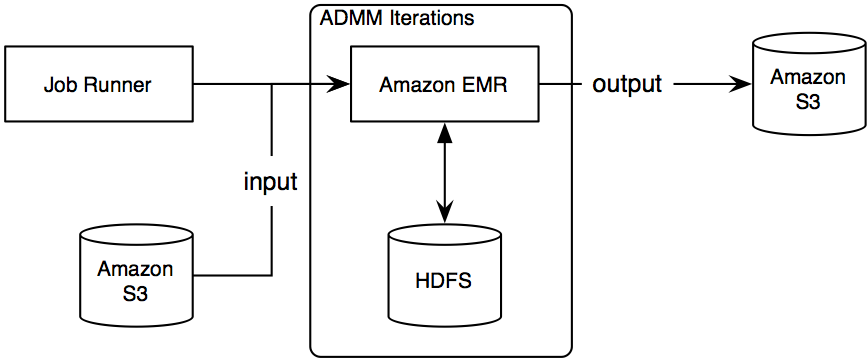
\includegraphics[width=3.2in]{aws_implementation}
\caption{The Job Runner sets paths for the input, the output data, and the Jar file with ADMM; it also sets any adjustable parameters, e.g. the number of iterations.  ADMM computes and stores intermediate data in HDFS, then after the final iteration, the $\hat{y}$ values ($z^k$ in ADMM notation) are output to S3.}
\label{fig:workflow}
\end{figure}

Wherever feasible, we have made our implementation of the ADMM algorithm generic.  Arguments to the driver allow users to exclude columns from the input data, optionally add an intercept, set the initial $\rho$, set the maximum number of iterations, and set the input and output locations. We have released an implementation of ADMM for Hadoop as an open source Java package.\footnote{\url{https://github.com/intentmedia/admm}}

\section{Results}\label{sec:results}
As part of our modeling pipeline, we run the ADMM algorithm daily on nearly a terabyte of data.  As depicted in Figure \ref{fig:workflow}, we load the data and a Jar file containing the ADMM algorithm from S3 and into EMR instances.  To evaluate the performance of our implementation of the ADMM algorithm, we examine the output of one day's run.  We measure performance by comparing the change in loss function per iteration.  We have also examined equivalent results from other days and saw that these results do not vary substantially from day to day.

Figure \ref{fig:iter} shows the difference between the predicted values and the actual values per iteration on a logarithmic scale.  The loss decreases, and therefore the accuracy consistently improves, as more iterations pass.  The steep decline at iteration 8 aligns with a substantial increase in the dual residual (not shown).  The dual residual equals
$$N\rho\|\bar{x}^k-\bar{x}^{k-1}\|^2_2,$$
which is the scaled step size between successive iterations. After iteration 8 we see an exponential decay in loss function for the subsequent iterations.  On a cluster of 20 high memory quadruple extra large EMR instances, 25 iterations run in 1 hour and 25 minutes.

\begin{figure}[!t]
\centering
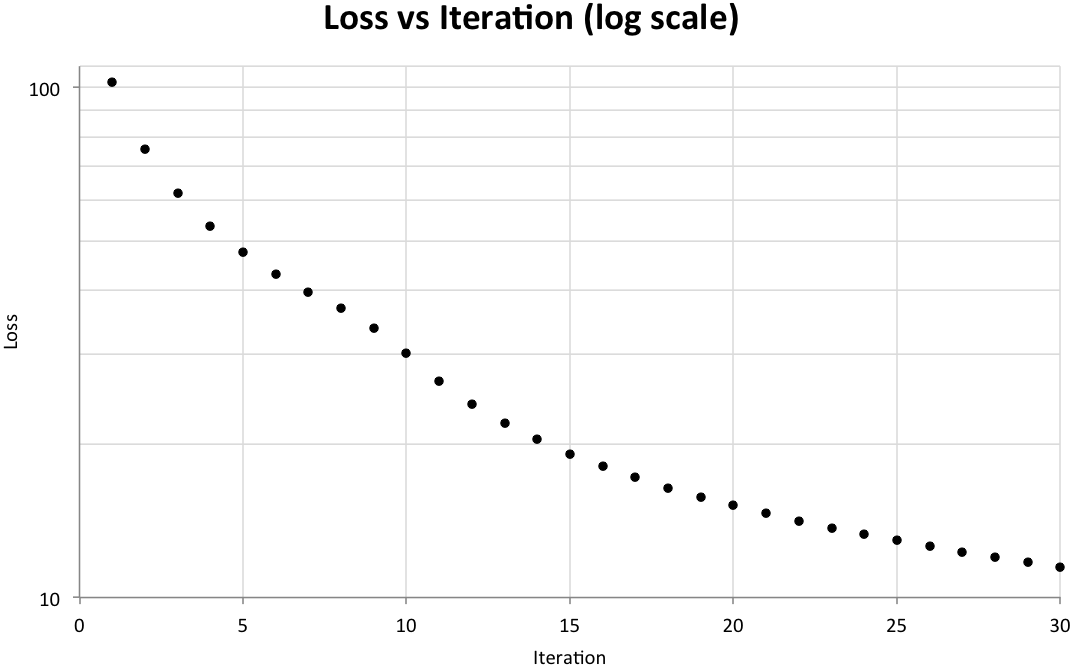
\includegraphics[width=3.2in]{iter_rnorm_plot}
\caption{Loss between our models predictions and the actual values per iteration on a logarithmic scale.  We see that the loss decreases dramatically and then decelerates during later iterations.}
\label{fig:iter}
\end{figure}

\section{Related Work}\label{sec:related}
The algorithm and our implementation are based upon \cite{boyd}, which introduced the ADMM algorithm.  \cite{bu2010} presents a more efficient approach to iterative computation in Hadoop requiring modifications to core Hadoop code, which reduce the time needed to transfer data and initialize MapReduce jobs.  This is not the approach we took as we stay within the Hadoop ecosystem and avoid the ramp-up costs associated with a less well known solution.  Based on our experience MapReduce is ``good enough'' for ADMM and logistic regression.  We evaluate the cost as described in \cite{lin2012}, and conclude that the reduction in implementation costs gained by using Hadoop outweigh the performance improvements that could be gained by using a less well-known platform. 

\cite{planet} presents a MapReduce implementation of tree ensemble learning and involves a wrapper for MapReduce that coordinates iterations of the underlying algorithm.  \cite{linkolcz2012} present a distributed method for classification that is similar to random forests. Apache Mahout contains an implementation of logistic regression that uses stochastic gradient descent (SGD).\footnote{https://cwiki.apache.org/MAHOUT/logistic-regression.html}  As noted in \cite{agarwal2011}, this SGD implementation is sequential, which substantially limits the performance of the algorithm and makes it difficult to scale.  To address this, \cite{agarwal2011} presents a scalable convex loss system that uses a Hadoop compatible variant of MapReduce.

\section{Conclusion}\label{sec:conc}
We have presented our implementation of the ADMM algorithm for Hadoop MapReduce.  Having an ADMM implementation allows us and other data scientists to more easily move our modeling ideas from prototype to production-scale.  We showed a specific example of using the ADMM algorithm to build a logistic regression model.  Importantly, ADMM is a general optimization algorithm that we can apply to other modeling problems with minimal modification.  Our contribution of a generic distributed optimization algorithm allows those using Hadoop to experiment with many different models at scale.
% conference papers do not normally have an appendix


% use section* for acknowledgement
%\section*{Acknowledgment}


%The authors would like to thank...
%more thanks here


% trigger a \newpage just before the given reference
% number - used to balance the columns on the last page
% adjust value as needed - may need to be readjusted if
% the document is modified later
%\IEEEtriggeratref{8}
% The "triggered" command can be changed if desired:
%\IEEEtriggercmd{\enlargethispage{-5in}}

% references section

% can use a bibliography generated by BibTeX as a .bbl file
% BibTeX documentation can be easily obtained at:
% http://www.ctan.org/tex-archive/biblio/bibtex/contrib/doc/
% The IEEEtran BibTeX style support page is at:
% http://www.michaelshell.org/tex/ieeetran/bibtex/
\bibliographystyle{IEEEtran}
% argument is your BibTeX string definitions and bibliography database(s)
\bibliography{pld_js_im_ieee_big_data}
%
% <OR> manually copy in the resultant .bbl file
% set second argument of \begin to the number of references
% (used to reserve space for the reference number labels box)



% that's all folks
\end{document}


